The TRITIUM-IFIC 0 prototype was the first prototype developed in TRITIUM experiment and it was used to check the feasibility of the technology proposed by TRITIUM, that's, to verify that it is possible to detect tritium in water using scintillating fibers.

Due to the problems that arise when liquid radioactive sources are used, the design of this first prototype paid special attention to radiation safety, rather than in detecting tritium efficiency.

The TRITIUM-IFIC 0 consists of bundle of 35 fibers, shown in Figure \ref{fig:FiberBundleOfTritiumIFIC0}, with a length of $20~\cm$, which were cut and polished with the techniques explained in section \ref{subsec:ConditioningProcess}. This bundle has a metalic pieze located in both ends, shown in Figure \ref{subfig:MetalicPieceFiberBunchTritiumIFIC0}, which are used to fix it to the prototype.

\begin{figure}[h]
 \centering
  \subfloat[Metalic piece of the fiber bundle]{
   \label{subfig:MetalicPieceFiberBunchTritiumIFIC0}
    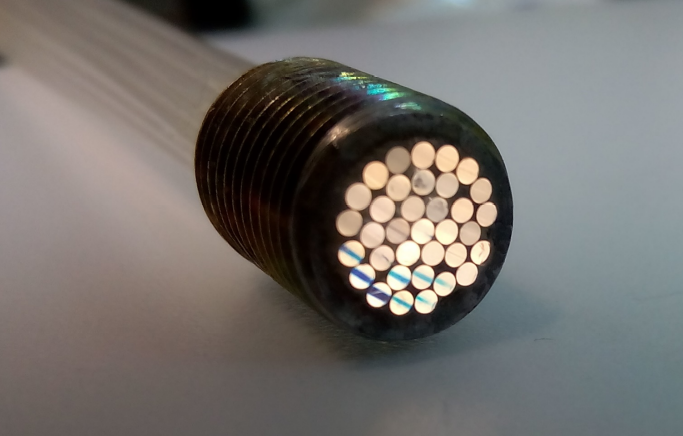
\includegraphics[angle=0, width=0.5\textwidth]{5Prototypes/52PreliminarPrototypes/521TritiumIFIC0/Metalic_piece_of_fiber_bundle.png}}
    %\newline
  \subfloat[Fiber bundle in a position similar to the prototype.]{
   \label{subfig:FiberBunchTritiumIFIC0Bent}
    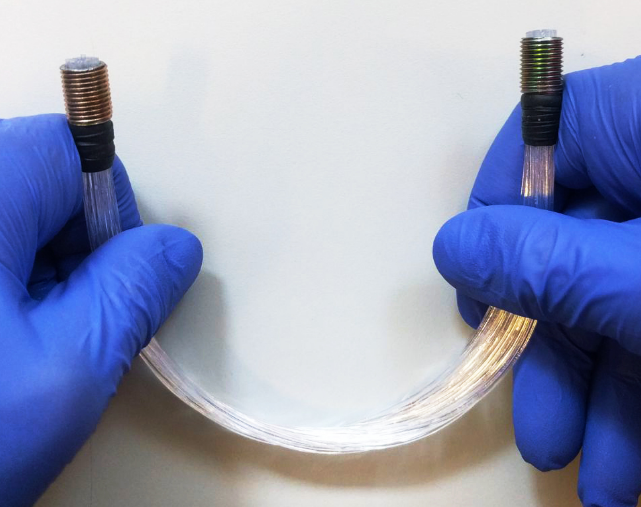
\includegraphics[angle=0, width=0.4\textwidth]{5Prototypes/52PreliminarPrototypes/521TritiumIFIC0/FiberBundleBent.png}}
    \newline
   \subfloat[Bundle of fibers in a straight position.]{
    \label{subfig:FiberBunchTritiumIFIC0}
     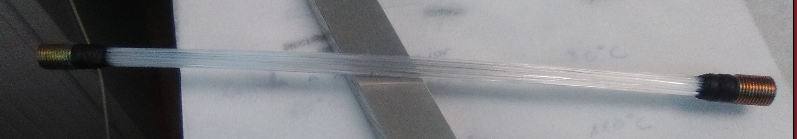
\includegraphics[angle=0, width=0.7\textwidth]{5Prototypes/52PreliminarPrototypes/521TritiumIFIC0/FiberBundleStraight.png}}
 \caption{Bundle of $35$ fibers, the length of which is $20~\cm$, used in TRITIUM-IFIC 0 prototype}
 \label{fig:FiberBundleOfTritiumIFIC0}
\end{figure}

This bundle is placed inside of a vessel, whose material is PVC\footnote{Polyvinyl Chloride, PVC}  since it is a safe material widely used. This vessel, shown in Figure \ref{fig:TritiumIFIC0}, was designed in a U-shape to improve the radiological safety, although this shape worsen the efficiency of tritium detection.

\begin{figure}[h]
\centering
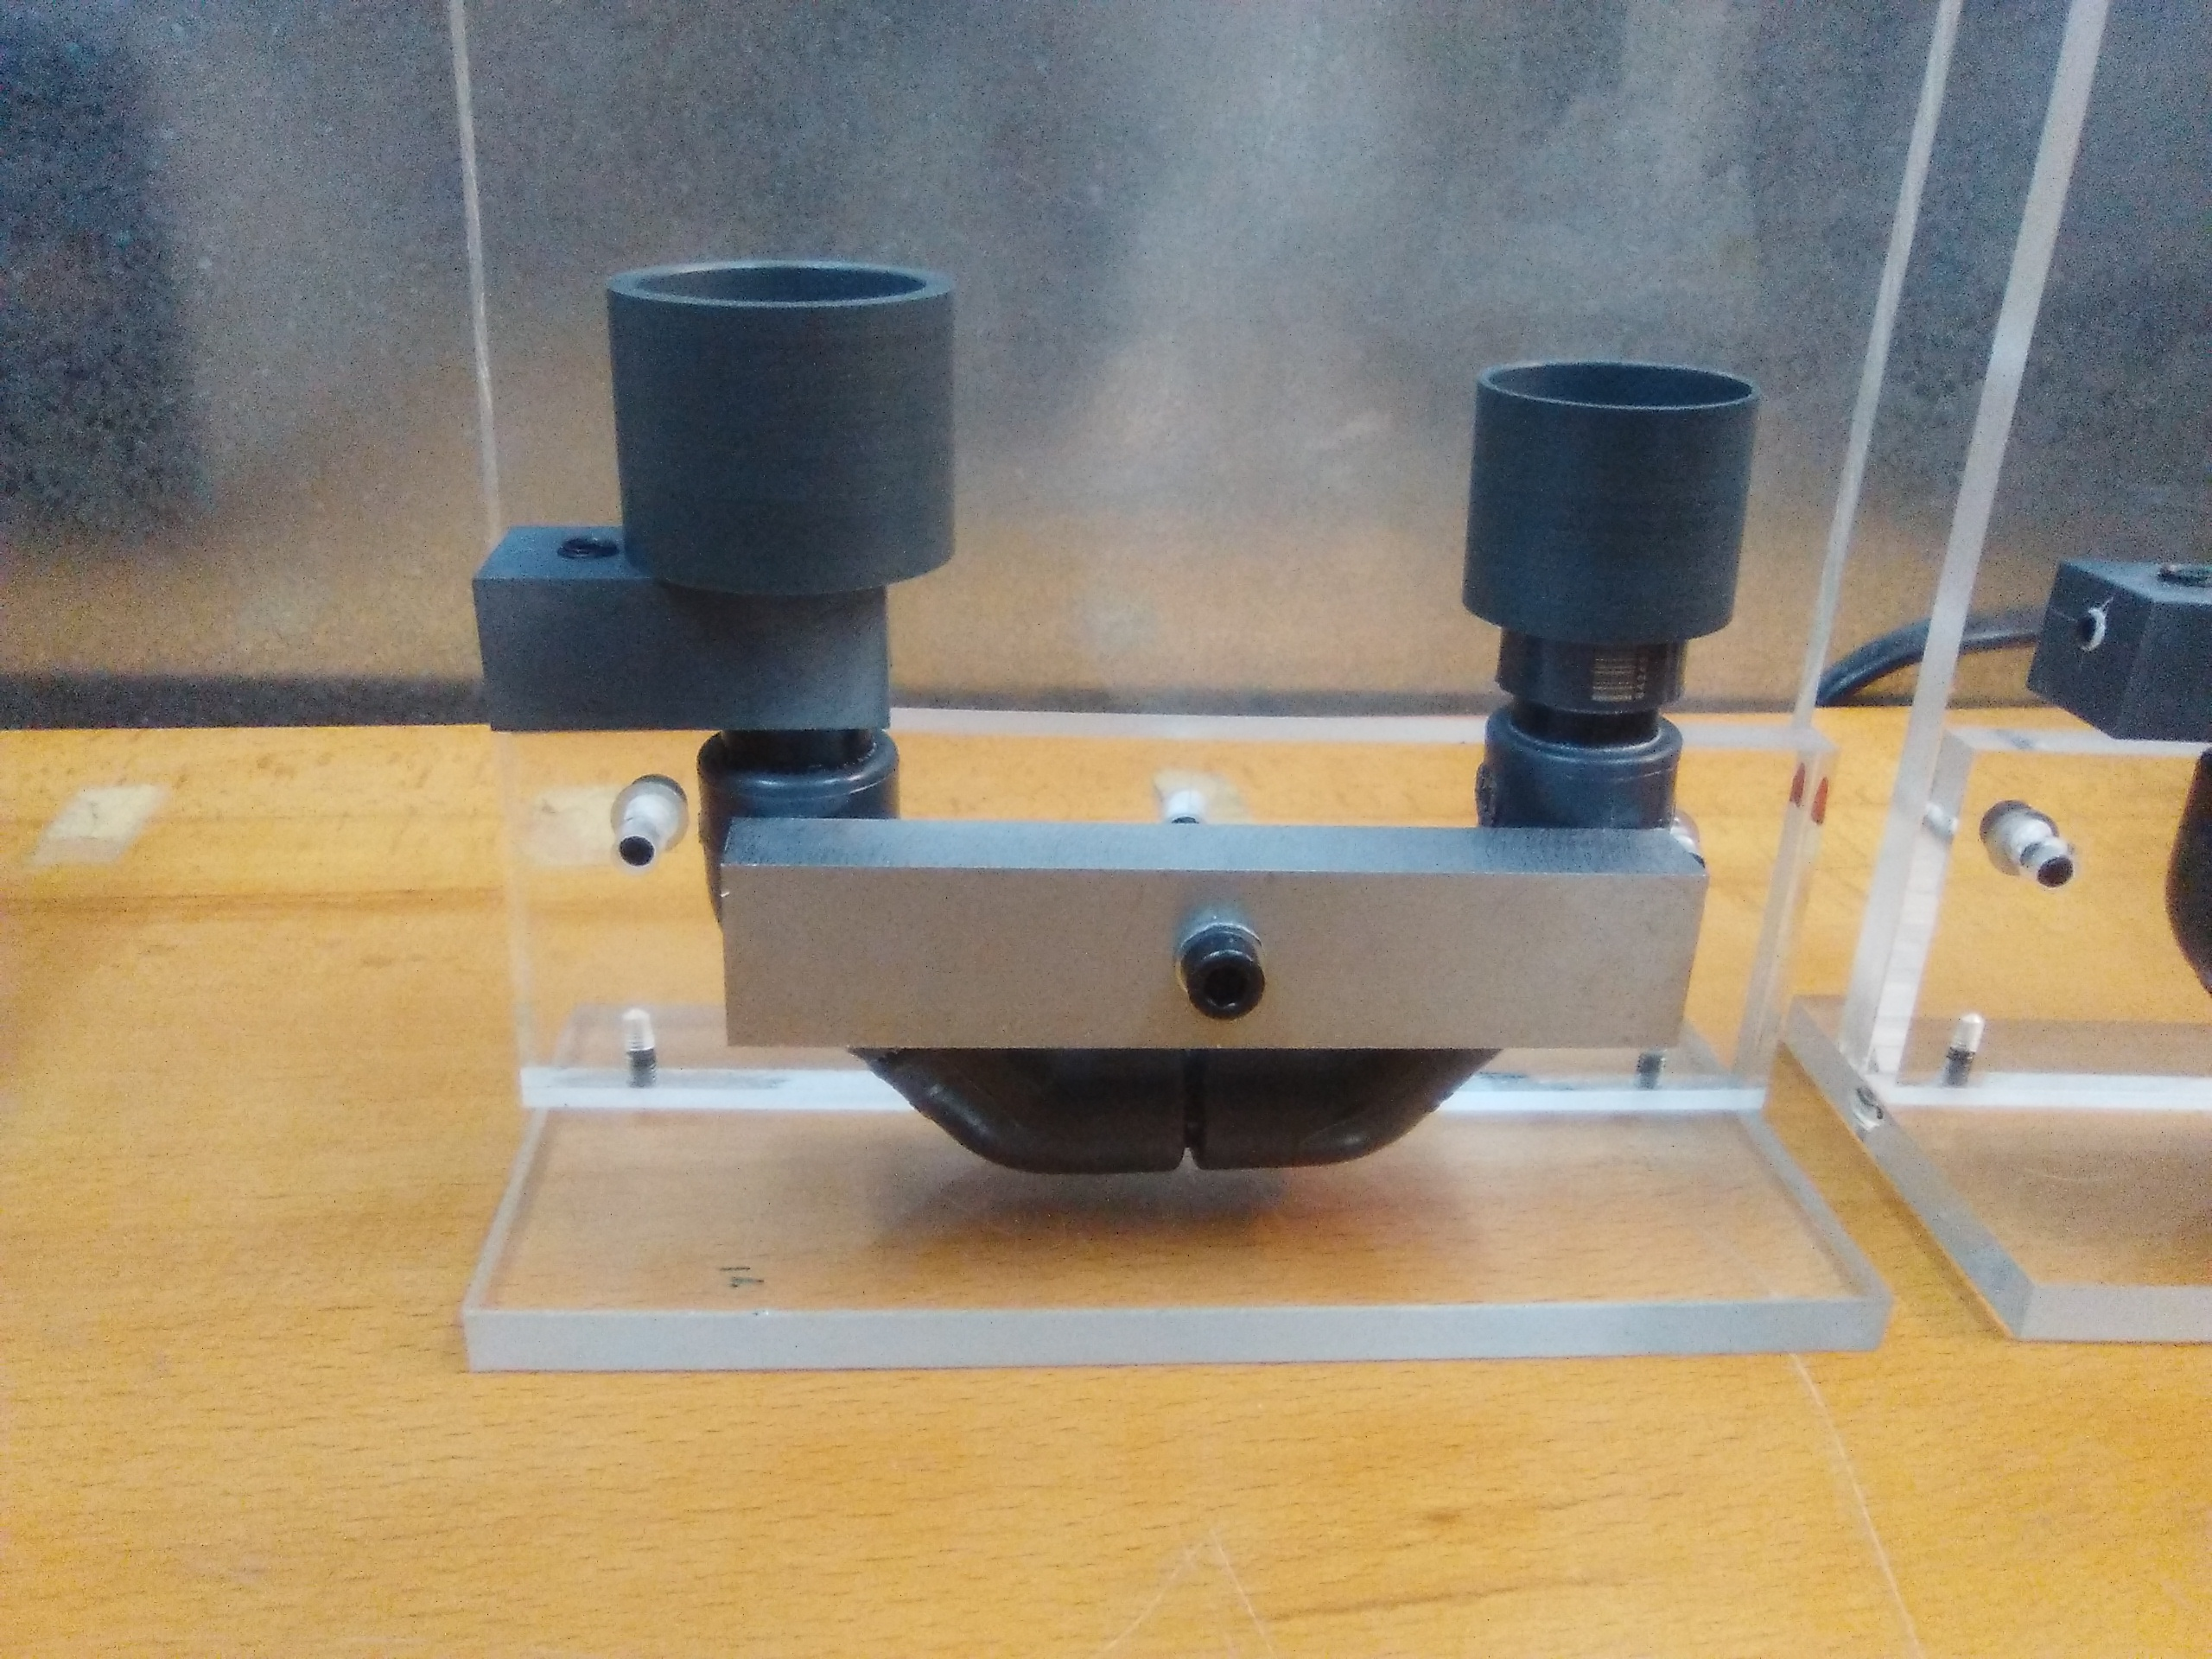
\includegraphics[scale=0.1]{5Prototypes/52PreliminarPrototypes/521TritiumIFIC0/Tritium_IFIC_0.jpg}
\caption{TRITIUM-IFIC 0 Prototype.\label{fig:TritiumIFIC0}}
\end{figure}

As can be seen in Figure \ref{fig:TritiumIFIC0}, a piece of methacrylate and steel was designed and built to hold the detector and two calibrated PMTs were optically coupled directly to the fiber bundle ends using optical grease \cite{OpticalGrease}.

The employed PMTs were the model R8520-460 from Hamamatsu company \cite{DataSheetPMTs}, whose reference number are ZB2771 and ZB2773, and the electronic circuit, shown in figure \ref{fig:VoltageDividerCircuit}, was used to distributed the high voltage between the dynodes. The employed high voltage was $-800~\volt$, at which their gain are $1.26 \cdot{} 10^6$ and $1.01 \cdot{} 10^6$ and their quantum efficiency are $29.76\%$ and $28.66\%$ respectively. Their signals were precessed and analyzed using the electronic configuration shown in Figure \ref{subfig:ElectronicConfiguraiton2PMT}.

Two identical prototypes were built and filled following the same protocol but ussing different liquid solutions. The first prototype, called TRITIUM-IFIC 0 Background, was filled only with  ultrapure water ($39~\cm^3$, uncertainty of $0.05\%$) and it was used to measure the radioactive background of the detector whereas the other prototype, called TRITIUM-IFIC 0 Signal, was filled with a radioactive liquid source of tritium, the preparation of which is explained in the appendix \ref{App:TritiumSourcePreparation}. The specific activity of the liquid source employed was $99.696~\kilo\becquerel/\liter$ (uncertainty of $2.24\%$) and the volume used to fill this prototype was the same as the other, $39~\cm^3$ (uncertainty of $0.05\%$). Therefore, the total activity of this tritiated water sample is approximately $3.888 \pm 0.087~\kilo\becquerel$. 

This second prototype was used to measure the signal of the detector (tritium + background) and the measured tritium activity can be known by extracting the background (measurement of TRITIUM-IFIC 0 Background) to the signal (measurement of TRITIUM-IFIC 0 Signal).

A statistically significant amount of time coincident events was not found in both PMTs, so the measurement of time coincidence was not possible. 

The loss of photons could be caused for several reasons, such as the poor quality of the tritiated water-fiber interface or the excessive curvature in the fiber bundle due to the U-shape of TRITIUM-IFIC 0 prototype, causing that too many photons escape from the fibers. The cleaning process explained in section \ref{subsec:CleaningProcess} was motivated by this result.

To avoid this problem and obtain some results with this prototype, a measurement was performed with a single PMT. For this task, the electronic configuration shown in Figure \ref{subfig:ElectronicConfiguraiton1PMT} was used. The results of these measurements are shown in section \ref{subsec:ResultsTritiumIFIC0}, where they are discussed.

In addition, a test was carried out to explain why it was not possible to measure both PMTs in time coincidence. For this task a transparent PMMA vessel, shown in Figure \ref{subfig:PMMAVesselToTestLostPhotons}, was built in a similar shape to that of the TRITIUM-IFIC 0 prototype vessel to check the effect of the fiber bundle curve. 

The LED shown in section \ref{subsubsec:CharacterizationFibers} was used to verify the reduction in photocollection efficiency of the fiber bundle due to this curve. 

\begin{figure}[h]
 \centering
  \subfloat[PMMA vessel]{
   \label{subfig:PMMAVesselToTestLostPhotons}
    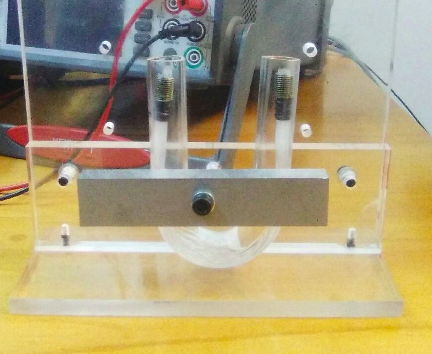
\includegraphics[angle=0, width=0.45\textwidth]{5Prototypes/52PreliminarPrototypes/521TritiumIFIC0/PMMA_vessel_ZOOM.png}}
    %\newline
  \subfloat[Test performed to check the lost photons.]{
   \label{subfig:TestLostPhotons}
    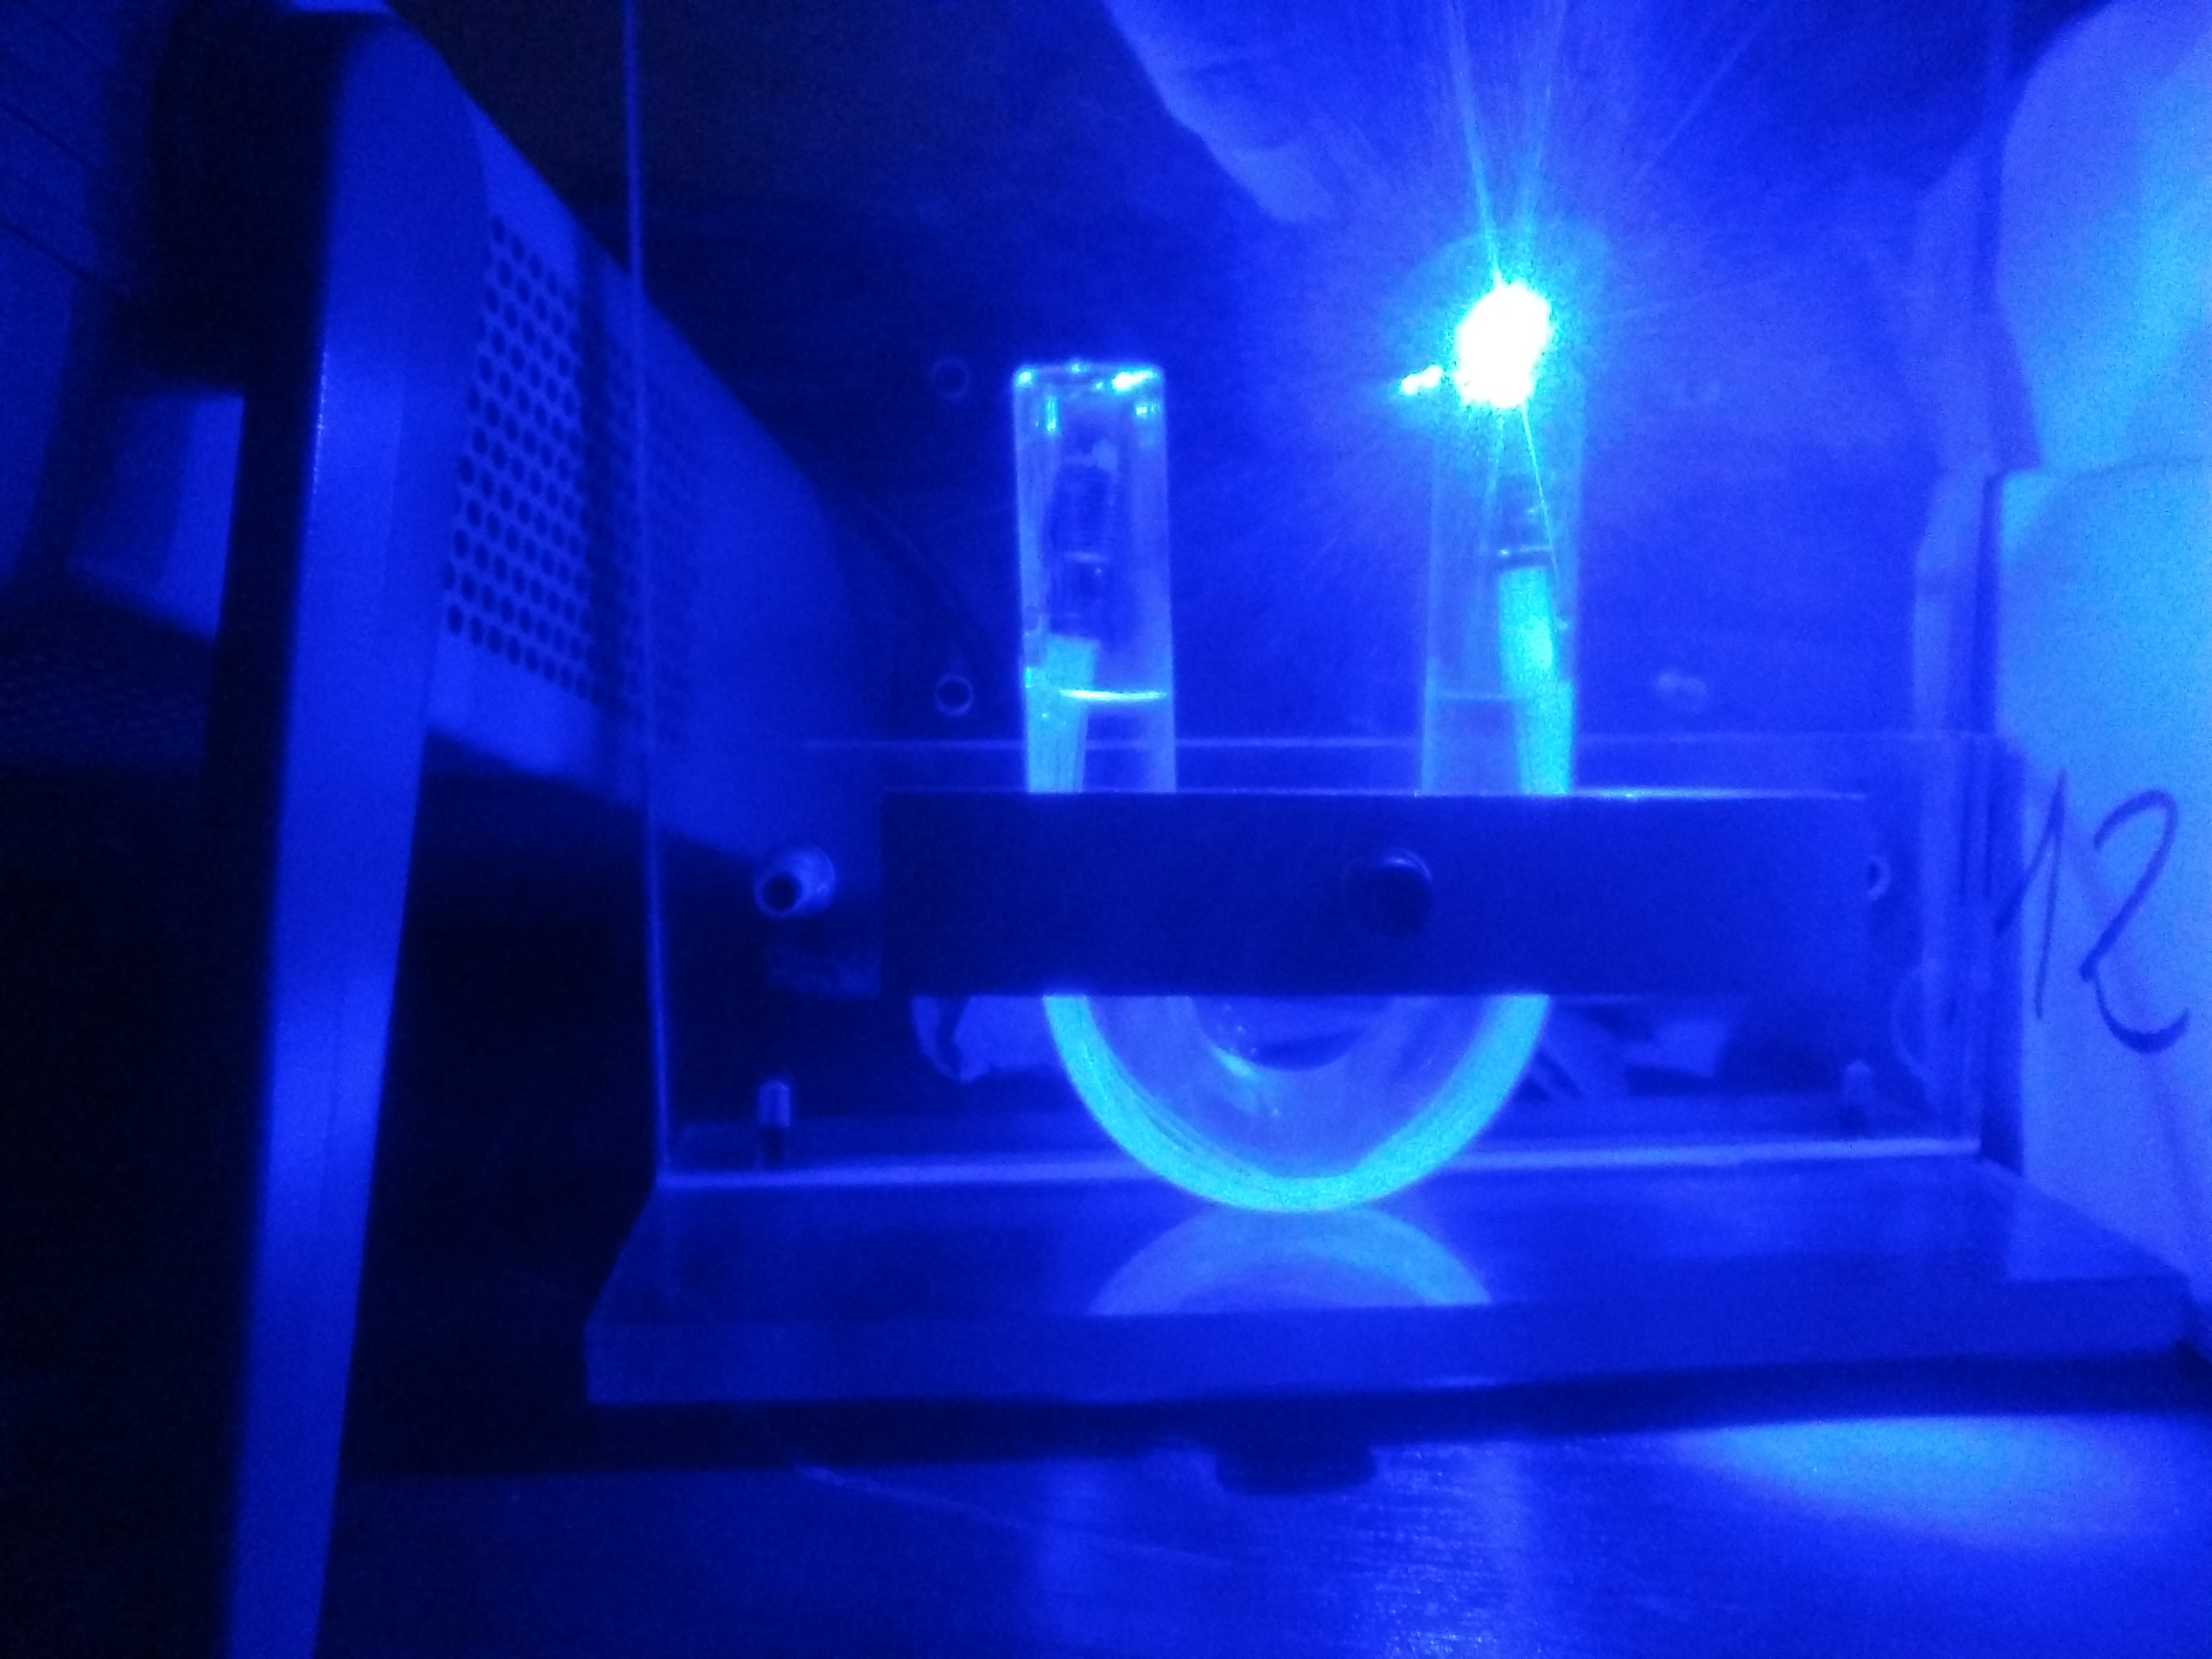
\includegraphics[angle=0, width=0.45\textwidth]{5Prototypes/52PreliminarPrototypes/521TritiumIFIC0/Lost_Photons.jpg}}
 \caption{PMMA vessel used to check photon loss due to fiber bundle curve.}
 \label{fig:TestLostPhotons}
\end{figure}

As can be seen visually in Figure \ref{subfig:TestLostPhotons}, a large percentage of the photons are lost due to the curve, which can be easily solved by using a straight fiber arrangement in next prototypes.

%In addition, some improvements was applied to next prototype, Tritium-IFIC 1. On the one hand, the special cleaning protocol, previously explained in section \ref{subsubsec:CleaningProcess}, was applied on the fibers. It was used to improve the interfaces between fiber and tritiated water, creating a better wetting property of the fiber, which will result in more tritium events detected and a greater photon collection efficiency.

%On the other hand, as we have seen in our previous characterization study of the fibers, shown in section \ref{subsubsec:CharacterizationFibers}, the photon collection efficiency of the fibers used is poor, so a large number of photons will be lost in each tritium event.

%It is an innerent characteristic of the fiber which we cannot change but, to reduce its effect, we will use a Teflon vessel for our next prototypes.

%Teflon is an interesting material for its optical properties, specifically its reflection factor, which is very close to $100\%$ at the working wavelength. It means that practically all the photons that reach the walls of the vessel will be reflected back to the fiber.

%On the other hand, the fibers were inspected under the electronic microscope of the SCSIE \cite{ElectronicMicroscopeSCSIE}, with which we can see details of the order of tens of nanometers.

%The result is shown in Figure \ref{}, where you can see many irregularities of the order of $X~\nm$. These irregularities will cause photons to escape from the fiber. It is a characteristic of the fibers that we cannot change but, to reduce its effect, we will use a Teflon vessel for our next prototypes.

%FOTOOOO

%Teflon is an interesting material for its optical properties, specifically its reflection factor. Its reflection factor is very close to $100\%$ at the working wavelength, which means that practically all the photons that reach walls of the vessel will be reflected back to the fiber.